\documentclass{article}

\usepackage{fullpage}
\usepackage{amsfonts}
\usepackage{graphicx}
\usepackage{lscape}
\usepackage{endfloat}

\newcommand{\beas}{\begin{eqnarray*}}
\newcommand{\enas}{\end{eqnarray*}}
\newcommand{\bea}{\begin{eqnarray}} \newcommand{\ena}{\end{eqnarray}}
\newcommand{\q}{k} \newcommand{\proof}{ {\bf Proof:} }
\def\squarebox#1{\hbox to #1{\hfill\vbox to #1{\vfill}}}
\newcommand{\qed}{\hfill\hfill\vbox{\hrule\hbox{\vrule\squarebox
{.667em}\vrule}\hrule}\smallskip} \newcommand{\level}{\mbox{$\theta$}}
\newcommand{\vspan}{\mbox{span}} \newcommand{\supp}{\mbox{supp}}
\newcommand{\trace}{\mbox{tr}} \newcommand{\real}{\mathcal Re}
\newcommand{\imag}{\mathcal Im} \newcommand{\diag}{\mbox{diag}}
\newcommand{\offd}{\mbox{off}} \newcommand{\low}{\mbox{low}}
\newcommand{\half}{{\frac{1}{2}}} \newcommand{\quarter}{{\frac{1}{4}}}
\newcommand{\eighth}{{\frac{1}{8}}} \newcommand{\Det}{\mbox{det}}
%\newcommand{\dim}{\mbox{dim}}
\newcommand{\Vscp}{V}
\newcommand{\rank}{\mbox{rank}}
\newcommand{\eig}{\mbox{{\bf eig}}}
\newcommand{\vect}{\mbox{vec}}
\newcommand{\integers}{\mbox{Z}}
\newcommand{\field}{\mathbb{F}}
\newcommand{\reals}{\mathbb{R}}
\newcommand{\complexes}{\mathbb{C}}
\newcommand{\nullspace}{Null}

\newcommand{\Rl}{\mathbb{R}}
\newcommand{\Nl}{\mathbb{N}}
\newcommand{\Ir}{\mathbb{Z}}
\newcommand{\Cx}{\mathbb{C}}
\newcommand{\A}{\mathcal{A}}
\newcommand{\HH}{\mathcal{H}}
\newcommand{\LL}{\mbox{ad}}
\newcommand{\KK}{\mathcal{K}}
\newcommand{\N}{\mathcal{N}}
\newcommand{\Proj}{{\rm Proj}}
\newcommand{\Span}{{\rm span}}
\newcommand{\abs}[1]{\lvert#1\rvert}
\newcommand{\floor}[1]{\left\lfloor{#1}\right\rfloor}
\newcommand{\ceil}[1]{\left\lceil{#1}\right\rceil}
\newcommand{\ket}[1]{\lvert#1\rangle}

\newtheorem{theorem}{Theorem}[section]
\newtheorem{definition}[theorem]{Definition}
\newtheorem{lemma}[theorem]{Lemma}
\newtheorem{corollary}[theorem]{Corollary}

\title{{\bf The Optimized Effective Potential with Finite Temperature}}

\author{Ross A. Lippert and N.~A. Modine}

\begin{document}

\maketitle

\begin{abstract}
The optimized effective potential OEP method provides an additional level
of exactness in electronic structures computations, e.g., the exact
exchange energy can be used.  This extra freedom is likely to be
important in moving density functional methods beyond traditional
approximations such as the local density approximation.  We provide
a new density-matrix-based derivation of the gradient of the Kohn-Sham
energy with respect to the effective potential.  This gradient can be
used to iteratively minimize the energy in order to find the OEP.
Previous work has indicated how this can be done in the zero temperature
limit.  This paper generalizes the previous results to the finite
temperature regime.  Equating our gradient to zero gives a finite-temperature
version of the OEP equation.
\end{abstract}

\section{Introduction}

The Kohn-Sham Density Functional Theory (DFT) \cite{KohnSham:65} has become one of the
most powerful tools for understanding and predicting the properties of materials.  DFT has
been applied to an ever increasing number of different types of systems and
phenomena, and the results have frequently been remarkably useful.  Nevertheless,
the accuracy of the results remains an important issue for many potential
applications of DFT.  The main source of error in DFT calculations is the use
of an approximate expression for the exchange-correlation energy, $E_{XC}$.
Such an approximation is necessary for practical calculations, but improving
the quality of the approximation, and hence, the accuracy of the calculations,
is of great interest.  Conventional variants of DFT, such as LDA and GGA, take
$E_{XC}$ to be an explicit functional of the electronic density.  Since the
noninteracting Kohn-Sham orbitals are implicit functionals of the electronic
density \cite{HohenbergKohn:64},  expressions for $E_{XC}$ that explicitly
depend on the Kohn-Sham orbitals are also consistent with the DFT framework.
An important example of such a functional is the functional used in the exact-exchange
approximation\cite{TalmanShadwick:76, SahniGruenebaumPerdew:82,EngelVosko:93,GorlingLevy:94,
Kotani:95,StadeleMajewskiVoglGorling:97,Gorling99}.  An explicit dependence
on the orbitals allows approximate $E_{XC}$ expressions to capture physical
behaviors of the exact Kohn-Sham $E_{XC}$ that can not be practically incorporated
in an expression that is an explicit function of only the electronic density.  One
example is the absence of self-interaction in the exact Kohn-Sham energy.
Another example is the complex, non-local behavior of the exact exchange energy.

The difficulty in using an $E_{XC}$ expression that is explicitly dependent on
the orbitals is that it is impossible to straightforwardly take the functional
derivative of $E_{XC}$ with respect to the electronic density.  Therefore,
standard self-consistent methods of minimizing the energy with respect to the
density can not be used.  The solution to this problem is provided by the
Optimized Effective Potential (OEP) formalism.  Since the energy is a functional
of the Kohn-Sham orbitals, and the orbitals are solutions of the Kohn-Sham
equation for some local potential, the energy can be viewed as a functional
of the potential.  The OEP is defined to be the potential that minimizes
the energy.  This minimization with respect to the potential is equivalent
to the usual minimization with respect to the density.  Traditionally, the OEP
has been calculated by solving the OEP integral equation, in which the gradient
of the energy with respect to the potential is set to zero \cite{TalmanShadwick:76,
SahniGruenebaumPerdew:82,EngelVosko:93,Kotani:95},
or by directly evaluating and inverting a response function \cite{GorlingLevy:94,
StadeleMajewskiVoglGorling:97,Gorling99}.

Two recent papers have proposed calculation of the OEP by means of an iterative minimization
of the energy \cite{HymanStilesZangwill:00,KummelPerdew:03}.  Hyman, Stiles, and Zangwill
used Lagrange multiplier methods to derive an expression for the gradient of the energy
with respect to the potential and proposed using this gradient to minimize the
energy iteratively.  Kummel and Perdew derived a nearly identical expression and,
although they did not claim that this expression gives the gradient, they noted
that it provides a good update to the potential during an iterative minimization.
In this paper, we present a new derivation of the gradient based on the
density matrix.  Our work goes beyond the previous papers in the following ways:
(1) We believe that our derivation is particularly transparent, and therefore,
it demonstrates that this expression is, in fact, the correct gradient.
(2)  The previous work assumed a negligible electronic temperature.  Since our
derivation is based on the density matrix, it is easily extended to finite
temperatures, where the orbitals are partially occupied.

One of the most exciting recent applications of DFT has been high energy density
physics.  In this application, electronic temperatures that are substantial
compared to the band gaps of typical semiconductors are common.  This makes
the results sensitive to the band gap, which is too small in the standard
versions of DFT. Therefore, the capability of performing calculations with
advanced functionals that have explicit dependence on the orbitals at
non-zero temperature is particularly exciting for high energy density physics
applications.

As an alternative to iterative minimization of the energy using the gradient,
it is possible, in principle, to find the OEP by solving the equation in
which the gradient is set to zero.  Therefore, our work provides the finite
temperature equivalent of the standard OEP equation, giving the correct
necessary condition for local optimality.

In this article, we derive the OEP method in a finite temperature regime
by considering the perturbation of the density matrix resulting from a
perturbed Hamiltonian.
The gradient will reduce to a combination of orbital shifts as one sees
in the zero temperature limit plus some corrections which come from the
finite temperature.  In section \ref{pert_sec}, we begin with a mathematical discussion
of the perturbation theory of analytic functions of Hermitian operators.
After a short review of density functional theory, we apply the results
of Section \ref{pert_sec} to the density matrix $\rho$ viewed as a function of
the Kohn-Sham Hamiltonian $H$, and thereby derive a finite temperature OEP
equation in terms of $H$ and $\rho$.   This motivates the subsequent
section, which describes the gradient expression in {\em orbital form}.
We conclude with some computational results demonstrating the accuracy
of the method.

\section{The perturbation theory of matrix-analytic functions}

\label{pert_sec}
Let $f(x)$ be an analytic function of $x$ and $f(A)$ be the
extension of $f$ to a matrix-analytic function
(see \cite{HornJohnson.book:91}, chapter 6) on some algebra of
Hermitian operators with a finite (or countable) spectrum.  Thus,
\bea
\label{com_eq}
 [A, f(A)] &=& A f(A) - f(A) A = 0\\
\label{eig_eq}
 f_i &=& f(a_i)
\ena
where the $a_i$ are the eigenvalues of $A$ and the $f_i$ are
the eigenvalues of $f(A)$.

For an unconstrained variation $A \rightarrow A + \delta A$
the variations of (\ref{com_eq}) and (\ref{eig_eq}) are
\bea
\label{dcom_eq}
 [\delta A, f(A)]+[A, \delta f(A)] &=& 0\\
\label{deig_eq}
 \delta f_i &=& f^\prime (a_i) \delta a_i.
\ena
In a basis where $A$ is diagonal
($a_i = A_{ii}, f(a_i) = \left[f(A)\right]_{ii}$),
(\ref{dcom_eq}) and (\ref{deig_eq}) become,
\bea
\label{ddcom_eq}
 (a_i - a_j) \left[\delta f(A)\right]_{ij} &=&  (f(a_i) - f(a_j)) \delta A_{ij}\\
\label{ddeig_eq}
 \delta \left[f(A)\right]_{ii} &=& f^\prime (a_i) \delta A_{ii}.
\ena
Thus (\ref{dcom_eq}) and (\ref{deig_eq})
appear to be sufficient to determine $\delta f(A)$ in terms of $A,\delta A$.

We may, somewhat informally, write the result as one equation
\bea
\label{jac_eq}
 \left[\delta f(A)\right]_{ij} &=& \frac{f(a_i) - f(a_j)}{a_i - a_j} \delta A_{ij}
\ena
where it is understood that we treat
$\frac{f(a_i) - f(a_j)}{a_i - a_j}$
as a {\em divided difference}, taking the limit as $a_i \rightarrow a_j$.

A more rigorous proof of these results can be made in the following theorem,
which also makes clear what happens in the presence of a repeated eigenvalue.
\begin{theorem}
The expansion of $f(A + \delta A) - f(A) = \delta f(A)$
 to first order in $\delta A$ is given by
%The expansion of $f(A + \delta A) - f(A) = \delta f(A) + \delta^2 f(A)$
% to second order in $\delta A$ is given by
\beas
\left[ \delta f(A) \right]_{ij} 
&=& \lim_{\epsilon\rightarrow 0}
     \frac{f(a_i+\epsilon) - f(a_j)}{a_i - a_j+\epsilon}
     \delta A_{ij} %\\
%\left[ \delta^2 f(A) \right]_{ij} 
%&=& 
% \lim_{\epsilon_1,\epsilon_2\rightarrow 0}
% \sum_{p}
%                 \frac{2}{a_i - a_j+\epsilon_1-\epsilon_2}
%		 \left(
%		    \frac{(a_i+\epsilon_1)^k - a_p^k}{a_i - a_p+\epsilon_1}
%		    -\frac{(a_j+\epsilon_2)^k - a_p^k}{a_j - a_p+\epsilon_2}
%		 \right)
%     \delta A_{ip} \delta A_{pj}
\enas
where the matrix elements are taken in an basis in which
$A$ is diagonal.
\end{theorem}
\proof
Since $f$ is analytic, it suffices to prove this theorem for
$f(x) = x^k$ and extend by linearity.

\beas
 \delta f(x) &=& \sum_{m+n=k-1} A^m \delta A A^n %\\
%             &=& \lim_{\epsilon_1,\epsilon_2 \rightarrow 0}
%                      \sum_{m+n=k-1} (A+\epsilon_1 I)^m \delta A (A+\epsilon_2 I)^n  %\\
% \delta^2 f(x) &=& 2 \sum_{l+m+n=k-2} A^l \delta A A^m \delta A A^n\\
%               &=& \lim_{\epsilon_1,\epsilon_2,\epsilon_3 \rightarrow 0}
%                   2 \sum_{l+m+n=k-2} (A+\epsilon_1 I)^l \delta A
%		                    (A+\epsilon_2 I)^m \delta A
%		                    (A+\epsilon_3 I)^n
\enas
in a diagonal basis,
\beas
 \left[\delta f(x)\right]_{ij}
             &=& \sum_{m+n=k-1} a_i^m a_j^n \delta A_{ij}\\
             &=& \sum_{m+n=k-1} \lim_{\epsilon\rightarrow 0} (a_i+\epsilon)^m a_j^n \delta A_{ij}\\
             &=& \lim_{\epsilon\rightarrow 0}
                 \frac{(a_i+\epsilon)^k - a_j^k}{(a_i+\epsilon) - a_j} \delta A_{ij} %\\
%             &=& \lim_{\epsilon_1,\epsilon_2 \rightarrow 0}
%                      \sum_{m+n=k-1} (a_i+\epsilon_1)^m (a_j+\epsilon_2)^n \delta A_{ij}\\
%             &=& \lim_{\epsilon_1,\epsilon_2 \rightarrow 0}
%		      (a_i+\epsilon_1)^{k-1}
%                      \sum_{n=0}^{k-1} \left(\frac{a_j+\epsilon_2}{a_i+\epsilon_1}\right)^{n}
%		      \delta A_{ij}\\
%             &=& \lim_{\epsilon_1,\epsilon_2 \rightarrow 0}
%                      \frac{(a_i+\epsilon_1)^k - (a_j+\epsilon_2)^k}
%			   {(a_i+\epsilon_1) - (a_j+\epsilon_2)}
%                      \delta A_{ij} %\\
% \left[\delta^2 f(x)\right]_{ij}
%               &=& \lim_{\epsilon_1,\epsilon_2,\epsilon_3 \rightarrow 0}
%                   2 \sum_{p,l+m+n=k-2} (a_i+\epsilon_1)^l
%		                    (a_p+\epsilon_2)^m 
%		                    (a_j+\epsilon_3)^n
%		   \delta A_{ip} \delta A_{pj}\\
%               &=& \lim_{\epsilon_1,\epsilon_2,\epsilon_3 \rightarrow 0}
%		 \frac{2}{(a_i+\epsilon_1) - (a_j+\epsilon_3)}
%		 \left(
%                      \frac{(a_i+\epsilon_1)^k - (a_p+\epsilon_2)^k}
%			   {(a_i+\epsilon_1) - (a_p+\epsilon_2)}
%                    - \frac{(a_j+\epsilon_3)^k - (a_p+\epsilon_2)^k}
%			   {(a_j+\epsilon_3) - (a_p+\epsilon_2)}
%		 \right)
%                 \delta A_{ip} \delta A_{pj},
\enas
and the summation is interchanged with the limit.
\qed

Note that one could clearly obtain higher order derivatives in terms of higher order
divided differences via the same approach.  To simplify forthcoming derivations,
we omit $\epsilon$'s and limits,
with the understanding that appropriate limits are to be taken for
divided differences of the form $\frac{f(x) - f(y)}{x-y}$.  We may interpret
(\ref{jac_eq}) as the equation which specifies the action of the {\em
Jacobian}, $\frac{\partial f(A)}{\partial A}$ on an arbitrary
Hermitian operator of the mapping $f$.

\subsection{Practical application of the Jacobian}

An $A$-diagonalizing basis might not be a convenient means to compute
the application of the Jacobian to an arbitrary variation.  We
present here a short digression on how such computations can be
carried out iteratively, without diagonalizing $A$.

We will be interested in applications of linear operators to Hermitian
(or anti-Hermitian) matrices.  To avoid some of the confusion entailed
in {\em operators of operators} discussions, we introduce some
notation, which we hope is clarifying.  We denote the application of a
linear operator on a matrix with brackets, $L\left[A\right]$.  In
terms of indices we may write this as $L\left[A\right]_{ij} = \sum_{kl} L_{ijkl} A_{kl}$.
For Hermitian matrices, we write $\left<X,Y\right> =
\trace\{XY\}$, and it is well known that this is a 
non-degenerate inner product on the vector space of Hermitian
matrices.  For a vector subspace of Hermitian matrices, $A$, we let
$A^\perp = \{B: \forall X\in A, \left<X,B\right>=0\}$.

We denote the linear action of a commutator $\LL_{X}\left[Y\right] = -\LL_{Y}\left[X\right] = [X,Y]$.
\begin{lemma}
\label{little_sym_lem}
\beas
\label{ad_transpose_eq}
 \left<X,\LL_Y[Z]\right> = -\left<\LL_{Y}[X],Z\right>.
\enas
\end{lemma}
\proof
Applying the trace identity $\trace\{AB\} = \trace\{BA\}$,
\beas
  \trace\{X (Y Z - Z Y)\}
  &=& \trace\{X Y Z - Y X Z\}\\
  &=& -\trace\{(Y X - X Y) Z\}
\enas
\qed

The {\em centralizer} of $X$ is the set $C_X =\{Y : [X,Y] = 0\}$.
$C_X$ is the nullspace of $\LL_X$.
\begin{lemma}
\label{range_lem}
$C_{X}^\perp$ is the range of $\LL_X$.
\end{lemma}
\proof
For any $Y$ and some $Z \in C_{X}$,
by lemma \ref{little_sym_lem},
$\left<\LL_{X}(Y),Z\right> = -\left<Y,\LL_{X}(Z)\right>=0$,
thus $\mbox{Range}\{\LL_{X}\} \subset C_{X}^\perp$.

From elementary dimension counting,
\beas
\dim\left\{ \mbox{Range}\{ \LL_X \} \right\} 
+ \dim\left\{ \mbox{Null}\{ \LL_X \} \right\}&=&
     \dim\{ C_{X} \} + \dim\{ C_{X}^\perp \} \\
\dim\left\{ \mbox{Range}\{ \LL_X \} \right\} 
+ \dim\left\{ C_X \right\}&=&
     \dim\{ C_{X} \} + \dim\{ C_{X}^\perp \} \\
\dim\left\{ \mbox{Range}\{ \LL_X \} \right\} 
   &=& \dim\{ C_{X}^\perp \} 
\enas
where $\dim\{ C_{X} \} = \dim\{ C_X \}$ obtains the
last line.
\qed

Let $X_{ij} = \frac{f(a_i) - f(a_j)}{a_i - a_j} Y_{ij}$ in an
$A$-diagonalizing basis.
Then according to (\ref{com_eq}) and (\ref{dcom_eq}),
\bea
\label{sparse_com_eq}
  \LL_A[X] &=& \LL_{f(A)}[Y].
\ena
The operator, $\LL_A$, has a non-trivial nullspace.
However, $C_A \subset C_{f(A)}$ implies $\mbox{Range}\{\LL_{f(A)}\}
\subset \mbox{Range}\{\LL_A\}$, by lemma \ref{range_lem}, thus equation 
(\ref{sparse_com_eq}) has a unique solution.

Since we are dealing with a linear space (albeit of matrices),
with a linear operator and an inner product, we can
use a Krylov-based iterative solver to solve (\ref{sparse_com_eq})
(e.g. conjugate gradient or MINRES \cite{minres,GolubVanLoan.book:89})
with some initial guess, $X_0$, yielding
\beas
  X = X_0 + c_1 \LL_A[X_0] +  c_2 \LL_A^2[X_0] + \cdots
\enas
with $X - X_0 \in C_A^\perp$.

By (\ref{deig_eq}), we additionally require $X_{ii} = f^\prime(a_i) Y_{ii}$.
For example, if we take
\beas
  X_0 = \half \left(f^\prime(A) Y + Y f^\prime(A) \right) + X_1,
\enas
where $X_1 \in C_A^{\perp}$ is arbitrary,
then the iterative solution of (\ref{sparse_com_eq}) will be correct,
i.e. $X = \delta f(A)$.  In the remainder of this article we take
$X_1 = 0$.

\section{Density functional theory review}

\label{dft_review}
Let $\rho$ be a density matrix (Hermitian),
$K$ be the kinetic energy operator, $V_{I}$ be the ionic (and
external) potential, with $E_{HXC}(\rho)$ the Hartree, exchange, and
correlation energy.  With
$S(P) =  - \trace\{ \rho \log(\rho) + (I-\rho) \log(I-\rho) \}$
as the entropy expression, the variational energy is
\bea
E(\rho) = \trace\{ \rho (K + V_I) \} + E_{HXC}(\rho) - \frac{1}{\beta} S(\rho).
\ena
The unconstrained derivative is 
\bea
\label{uncon_deriv_eq}
\frac{\partial E}{\partial \rho} &=&
 K + V_I + \frac{\partial E_{HXC}}{\partial \rho} +
 \frac{1}{\beta} \log(\rho(I-\rho)^{-1}).
\ena

The Kohn-Sham Hamiltonian is given by $H = K + V_I + \Vscp$ where
$\Vscp$ is the self-consistent potential (to be determined).
In the Kohn-Sham DFT, $\rho$ is the minimizer of
$\trace\{\rho H \} - \frac{1}{\beta} S(\rho)$
with $\trace\{\rho\}=n$, which is equivalent to the conditions,
\bea
\label{rho_eq}
  \rho &=& \frac{1}{1+e^{\beta (H - \mu I)}} = f_\beta(H-\mu I)\\
\label{trace_rho_eq}
  \trace\{\rho\} &=& n
\ena
for some chemical potential $\mu$.
Thus, we can consider $\rho$ to be parametrized by two unknowns
$\Vscp$ and $\mu$ with two relations (\ref{rho_eq}) and (\ref{trace_rho_eq}).
Note: one could absorb $\mu$ into $\Vscp$, but we find it
advantageous to keep it distinct in its role as a Lagrange multiplier.

With $\rho$ satisfying these relations, the energy differential simplifies
\beas
\frac{\partial E}{\partial \rho}
 &=&
 K + V_I + \frac{\partial E_{HXC}}{\partial \rho} +
 \frac{1}{\beta} \log(\rho(I-\rho)^{-1})\\
 &=&
 K + V_I + \frac{\partial E_{HXC}}{\partial \rho} 
 - (H - \mu I)\\
 &=& 
  \frac{\partial E_{HXC}}{\partial \rho} 
 - (\Vscp - \mu I).
\enas
\label{dft_review_sec}

\section{Finite temperature OEP with density operators}

From section \ref{dft_review_sec}, the density matrix is
related to the Kohn-Sham Hamiltonian, $H$, by (\ref{rho_eq}) and (\ref{trace_rho_eq}).
Let $\varepsilon_i$ be the eigenvalues of $H$, and let
$\omega_i = f_\beta (\varepsilon_i-\mu)$ be the eigenvalues of $\rho$.
The divided differences can be stably computed with the formula
$$\frac{f_{\beta}(x) - f_{\beta}(y)}{x-y} =
  -\frac{e^{\beta (x+y)/2}}{(1+e^{\beta x})(1+e^{\beta y})}
  \left(\frac{\mbox{sinh}(\beta (x-y)/2)}{(x-y)/2}\right)
$$
where a test for $x=y$ is required for the evaluation of
the last factor.  We note in particular that
$\frac{f_\beta(x)-f_\beta(x)}{x-x} = 
\frac{d}{dx}f_\beta(x) = -\beta f_\beta(x)(1-f_\beta(x))$.

Let $E(\rho)$ be a function of a density matrix, $\rho$.
We can implicitly define $E(H) = E(\rho(H,\mu(H)))$.
Formally varying $E(H)$,
\bea
\label{pre_dE_eq}
 \delta E(H) =
     \trace\left\{
     \frac{\partial E(\rho(H,\mu))}{\partial \rho} \delta \rho
     \right\}.
\ena
in an $H$-diagonalizing basis,
\bea
\label{diag_drho_eq}
 \delta \rho_{ij} = \frac{\omega_i - \omega_j}{\varepsilon_i-\varepsilon_j}
               \left( \delta H_{ij} - \delta \mu \delta_{ij} \right).
\ena
By (\ref{trace_rho_eq}), the trace of $\delta \rho$ vanishes,
\beas
 \delta \mu 
   &=& 
    \frac{\sum_{ij}
      \delta_{ij} \frac{\omega_i - \omega_j}{\varepsilon_i-\varepsilon_j} \delta H_{ij}
    }{\sum_{ij}
      \delta_{ij} \frac{\omega_i - \omega_j}{\varepsilon_i-\varepsilon_j}
    }\\
   &=& \frac{ \trace\{ \rho(I-\rho)\delta H \} }
         { \trace\{ \rho(I-\rho) \} }.
\enas
Thus, in an $H$-diagonalizing basis,
\beas
 \delta E
&=& \sum_{ij}
       \frac{\partial E}{\partial \rho_{ij}} 
       \frac{\omega_i - \omega_j}{\varepsilon_i-\varepsilon_j}
        \left( \delta H_{ij} - \delta \mu \delta_{ij} \right)\\
&=& \sum_{ij}
       \frac{\partial E}{\partial \rho_{ij}} 
       \frac{\omega_i - \omega_j}{\varepsilon_i-\varepsilon_j}
       \left(
       \delta H_{ij}
               -
       \frac{\sum_k \omega_k(1-\omega_k) \delta H_{kk} }
	     {\sum_k \omega_k (1 - \omega_k)}
       \delta_{ij}
       \right)\\
&=&
    \sum_{ij}
    \left(
       \frac{\omega_i - \omega_j}{\varepsilon_i-\varepsilon_j}
       \frac{\partial E}{\partial \rho_{ij}} 
               -
       \delta_{ij}
         \frac{\omega_i(1-\omega_i)}{\sum_k \omega_k (1 - \omega_k)}
    \sum_{pq}  \delta_{pq}
         \frac{\omega_p - \omega_q}{\varepsilon_p-\varepsilon_q}
              \frac{\partial E}{\partial \rho_{pq}}
       \right)       \delta H_{ij}
\enas
and the gradient is therefore
\bea
\label{diag_grad_eq}
 \frac{\partial E}{\partial H_{ij}}
  &=&
       \frac{\omega_i - \omega_j}{\varepsilon_i-\varepsilon_j}
       \frac{\partial E}{\partial \rho_{ij}} 
               -
       \delta_{ij}
         \frac{\omega_i(1-\omega_i)}{\sum_k \omega_k (1 - \omega_k)}
    \sum_{pq}  \delta_{pq}
         \frac{\omega_p - \omega_q}{\varepsilon_p-\varepsilon_q}
              \frac{\partial E}{\partial \rho_{pq}}\\
\label{nodiag_grad_eq}
\frac{\partial E}{\partial H}
  &=& \frac{\Delta \omega}{\Delta \varepsilon}
       \left[\frac{\partial E}{\partial \rho}\right]
       -
       \frac{\rho(I-\rho)}
	    {\trace\{ \rho (I-\rho) \} }
       \trace\left\{\frac{\Delta \omega}{\Delta \varepsilon}
               \left[\frac{\partial E}{\partial \rho}\right]\right\}\\
\label{nodiag_grad_eq2}
  &=& \frac{\Delta \omega}{\Delta \varepsilon}
       \left[\frac{\partial E}{\partial \rho} - 
       \frac{ \trace\left\{\frac{\Delta \omega}{\Delta \varepsilon}
               \left[\frac{\partial E}{\partial \rho}\right]\right\} }
	    { \trace\left\{\frac{\Delta \omega}{\Delta \varepsilon}
              \left[ I \right]\right\} }
	    I
       \right]
\ena
where $\frac{\Delta \omega}{\Delta \varepsilon}\left[\cdot\right]$ stands for
the Jacobian, $\frac{\omega_i - \omega_j}{\varepsilon_i-\varepsilon_j}$,
in a general basis.
$\trace\left\{\frac{\Delta \omega}{\Delta \varepsilon}\left[ I \right]\right\}
= -\beta \trace\{\rho(I-\rho)\}$, though we will keep it as it is in
(\ref{nodiag_grad_eq2}) to make the tracelessness of $\frac{\partial E}{\partial H}$
more manifest.

The application of the Jacobian, to obtain
$\frac{\partial E}{\partial H} = \frac{\Delta \omega}{\Delta \varepsilon}
       \left[\frac{\partial E}{\partial \rho} - 
       \frac{ \trace\left\{\frac{\Delta \omega}{\Delta \varepsilon}
               \left[\frac{\partial E}{\partial \rho}\right]\right\} }
	    { \trace\left\{\frac{\Delta \omega}{\Delta \varepsilon}
              \left[ I \right]\right\} }
	    I
       \right]$,
%$\frac{\Delta \omega}{\Delta \varepsilon}\left[\frac{\partial E}{\partial \rho}\right]$,
can be done by iteratively solving
\bea
\label{DFT_com_eq}
  \left[H,\frac{\partial E}{\partial H} \right]
  = \left[\rho, \frac{\partial E}{\partial \rho}\right]
\ena
with initial guess
\bea
\label{DFT_init_eq}
  \left(\frac{\partial E}{\partial H}\right)_0 &=& 
   -\half \beta \left(
      \rho (I - \rho) \frac{\partial E}{\partial \rho}
    + \frac{\partial E}{\partial \rho} \rho (I - \rho)
  \right)
  + \beta
  \frac{ \trace\left\{\frac{\Delta \omega}{\Delta \varepsilon}
               \left[\frac{\partial E}{\partial \rho}\right]\right\} }
	    { \trace\left\{\frac{\Delta \omega}{\Delta \varepsilon}
              \left[ I \right]\right\} }
   \rho(I - \rho)        .
\ena
Note:
$\lim_{\beta \rightarrow \infty} \beta \rho (I-\rho) \propto \delta(H - \mu I)$,
a delta function on the spectrum of $H$.  Thus in the low temperature limit,
only the eigenvalues of $H$ near $\mu$ contribute to
$\left(\frac{\partial E}{\partial H}\right)_0$.

%It is also worth noting here the asymptotic behavior of the individual
%$\frac{\partial E}{\partial H_{ij}}$ in an $H$-diagonal basis.
%\beas
% \lim_{\omega_i,\omega_j \rightarrow 1}\frac{\partial E}{\partial H_{ij}}&=&0\\
% \lim_{\omega_i,\omega_j \rightarrow 0}\frac{\partial E}{\partial H_{ij}}&=&0,
%\enas
%thus, we see that as $\beta\rightarrow \infty$, the couplings are
%between occupied and unoccupied eigenstates of $H$.  Similarly, we
%see that for finite $\beta$ as $\varepsilon_i,\varepsilon_j \rightarrow \infty$
%the coupling between states $i$ and $j$ vanishes.  These vanishing couplings
%are of great importance when translating these results to an orbital
%representation.

To obtain an OEP gradient, we restrict the
variability of $H$ to $H = H_0 + \Vscp$ where $H_0 = K + V_{I}$ is fixed and $\Vscp$ is a
local operator.  The gradient is then
\bea
\label{dEdV_eq}
 \frac{\partial E}{\partial V(r)} 
     &=& \sum_{ij} \phi_i(r) 
         \frac{\partial E}{\partial H_{ij}} \phi_j^*(r)
\ena
where $\phi_i(r)$ is the eigenvector of $H$ with eigenvalue $\varepsilon_i$
in the position representation.

\label{density_sec}


\section{Finite temperature OEP with orbitals}

Instead of representing the density as an operator, it is often
more practical to express $\rho$ in terms of an incomplete basis
of partially occupied orbitals.
Let $\phi_1,\phi_2,\ldots$ be a complete eigenbasis of $H$
sorted non-decreasingly in eigenvalue.  Let $N$ be sufficiently
large that $\omega_{i > N} \sim 0$.  Then we may write truncate
the basis so that
\bea
  \rho = \phi \Omega \phi^\dagger
\ena
where $\phi = \left[ \matrix{ \phi_1 & \phi_2 & \cdots & \phi_N }\right]$,
with $\Lambda$ the diagonal matrix of eigenvalues and
$\Omega$ the diagonal matrix with entries $\omega_1,\ldots,\omega_N$
(i.e. $\Omega = f_\beta(\Lambda - \mu I)$).  Note, $N$ will
usually be much smaller than the number of primitive basis functions, so
$\phi$ will be a rectangular matrix with orthonormal columns,
i.e. $\phi^\dagger \phi = I$ (the $N \times N$ identity)
and $\phi \phi^\dagger$ is the orthogonal projector
onto the span of the $\phi_i$ (and hence commutes with $H$).

Let $\chi$ and $\zeta$ be given by
\beas
\chi &=& \trace\left\{\frac{\Delta \omega}{\Delta \varepsilon}
               \left[\frac{\partial E}{\partial \rho}\right]\right\}
  = \sum_{i\ge 1} -\beta \omega_i (1-\omega_i)
    \phi_i^\dagger\frac{\partial E}{\partial \rho}\phi_i\\
\zeta &=& \trace\left\{\frac{\Delta \omega}{\Delta \varepsilon}\left[I\right]\right\}
  = \sum_{i\ge 1} -\beta \omega_i (1-\omega_i)
\enas
and let $\bar{E}$ and $\bar{J}$ be $N\times N$ matrices given by
\bea
\label{Ebar_def_eq}
%\bar{E}_{ij} &=&
% \phi_i^\dagger \frac{\partial E(\phi \Omega \phi^\dagger)}{\partial \rho} \phi_j
%=
% \frac{\partial E(\phi \Omega \phi^\dagger)}{\partial \rho_{ij}}
\bar{E} =
 \phi^\dagger \frac{\partial E(\phi \Omega \phi^\dagger)}{\partial \rho} \phi
&\quad& \left( \mbox{i.e. }
\bar{E}_{ij} =
 \frac{\partial E(\phi \Omega \phi^\dagger)}{\partial \rho_{ij}}\right)
\\
\label{Jbar_def_eq}
%\bar{J}_{ij} &=&
% \phi_i^\dagger 
%   \frac{\Delta \omega}{\Delta \varepsilon} \left[
%        \frac{\partial E}{\partial \rho}
%  - \frac{\chi}{\zeta} I
%   \right]
%   \phi_j
% =
% \frac{\omega_i - \omega_j}{\varepsilon_i - \varepsilon_j} 
%  \left(\bar{E}_{ij} - \frac{\chi}{\zeta}\delta_{ij}\right).
\bar{J} =
 \phi^\dagger 
   \frac{\Delta \omega}{\Delta \varepsilon} \left[
        \frac{\partial E}{\partial \rho}
  - \frac{\chi}{\zeta} I
   \right]
   \phi
&\quad& \left( \mbox{i.e. }
\bar{J}_{ij} =
 \frac{\omega_i - \omega_j}{\varepsilon_i - \varepsilon_j} 
  \left(\bar{E}_{ij} - \frac{\chi}{\zeta}\delta_{ij}\right)
\right).
\ena
Note that by these definitions,
$\left[\Omega,\bar{E}\right] = \left[\Lambda,\bar{J}\right]$.

Since $\omega_{i>N} \sim 0$, the expressions for $\chi$ and
$\zeta$ can likewise be truncated,
\beas
\chi &=& \sum_{1\le i \le N} -\beta \omega_i (1-\omega_i) \bar{E}_{ii}
      = -\beta \trace\left\{ \Omega(I-\Omega) \bar{E} \right\}\\
\zeta &=& \sum_{1\le i \le N} -\beta \omega_i (1-\omega_i)
      = -\beta \trace\left\{ \Omega(I-\Omega) \right\}\\
\enas
and by (\ref{diag_grad_eq})
\beas
(I-\phi \phi^\dagger)
   \frac{\Delta \omega}{\Delta \varepsilon} \left[
        \frac{\partial E}{\partial \rho} - \frac{\chi}{\zeta} I\right]
(I - \phi \phi^\dagger) = 0,
\enas
thus, we may write (\ref{nodiag_grad_eq}) as
\bea
\label{orb_jacE_eq}
\frac{\partial E}{\partial H} &=&
\frac{\Delta \omega}{\Delta \varepsilon} \left[
    \frac{\partial E}{\partial \rho} - \frac{\chi}{\zeta} I\right] =
  \phi \psi^\dagger + \psi \phi^\dagger,
\ena
where $\phi^\dagger \psi = \psi^\dagger \phi = \half \bar{J}$.
This gives an orbital form of equation (\ref{dEdV_eq}),
\bea
\label{new_oep_eq}
\frac{\partial E}{\partial V(r)}
     &=& \sum_{1\le i\le N} \phi_i(r) \psi_i^*(r)+\psi_i(r) \phi_i^*(r)
\ena
which is similar to the equation derived in numerous sources in the OEP
literature \cite{HymanStilesZangwill:00,KummelPerdew:03}, with a modification of the $\psi$ to
accommodate the finite temperature regime.

It remains to solve for $\psi$, which we may decompose as
$\psi = \psi_{\perp}+\half \phi \bar{J}$,
where $\phi^\dagger \psi_{\perp}=0$.
We can derive an equation for $\psi_{\perp}$,
by multiplying equation (\ref{DFT_com_eq})
on the left by the projector
$I - \phi \phi^\dagger$ (which commutes with $H$) and on the
right by $\phi$ and employing (\ref{orb_jacE_eq}),
\bea
 (I-\phi \phi^\dagger)
 \left[H,\frac{\partial E}{\partial H}\right] \phi 
  &=&
 (I-\phi \phi^\dagger)
 \left[\rho, \frac{\partial E}{\partial \rho}\right]\phi
\\
 (I-\phi \phi^\dagger)
 \left(H \psi - \psi \Lambda\right)
  &=&
 -(I - \phi \phi^\dagger) \frac{\partial E}{\partial \rho} \rho \phi
\\
\label{final_eq}
 H \psi_{\perp} - \psi_{\perp} \Lambda
  &=&
 -(I - \phi \phi^\dagger) \frac{\partial E}{\partial \rho} \phi \Omega.
\ena
The LHS and RHS of (\ref{final_eq}) are orthogonal to $\phi$,
by construction.
Thus we have a well-defined
equation for $\psi_{\perp}$.
%We can solve for $\bar{J}$ in the $\phi$ basis by diagonalization.
An iterative method can thus be used to solve for $\psi_{\perp}$ without any
special initialization beyond $\phi^\dagger \psi_{\perp} = 0$.


\section{Computational results}

In order to test the above approach, it was implemented in the orbital representation
within the Socorro electronic
structure software using a plane wave basis set and norm-conserving pseudopotentials.
The conjugate gradient algorithm was used to solve the linear systems involved in the
evaluation of the gradient.  Using this algorithm, the computational cost of solving
the set of linear systems determining $\psi_{\perp}$ is comparable to the cost of
solving the Kohn-Sham eigenproblem for $\phi$.  Therefore, each gradient evaluation
is approximately as computationally expensive as one step of the self-consistency
loop in a standard DFT code.

For traditional approximations to the exact DFT,
such as the Local Density Approximation (LDA) and Generalized Gradient Approximation (GGA),
$E_{HXC}$ is an explicit functional of the electronic density, which is the diagonal of
the density matrix $\rho$ in a position representation.  In this case,
$\frac{\partial E_{HXC}}{\partial \rho}$ has the form of a local potential operator $V_{HXC}$,
and the energy minimum occurs at self-consistency, i.e., when $\Vscp = V_{HXC}$.
In this case, the OEP is the self-consistent potential, and the results of our iterative
minimization approach can be compared directly to well-tested results obtained from
conventional self-consistent methods.  Therefore, we have tested our OEP approach by applying
it to LDA calculations.

Our test system consists of a two atom unit cell of silicon in the diamond structure.  We used a
20 Rydberg plane-wave cutoff and a $2 \times 2 \times 2$ Monkhorst-Pack k-point sampling.
This k-point sampling does not give a converged total energy, but this is not an issue for
the purpose of testing our approach.  Two electronic temperatures were used: (1) Room Temperature
($k_B T = 25.67$ meV), and (2) High Temperature ($k_B T = 1.0$ eV).

\begin{figure}[p]
\includegraphics[height=5in]{Figure_1.ps}
\caption{A comparison of the energy change predicted from the gradient
and the actual energy change observed during a random walk in the
potential.  The filled circles are the calculated values.  The solid
line is a guide to the eye representing perfect agreement.}
\label{fd_test}
\end{figure}

In order to test the correctness of the our gradient, we used the finite difference approach.
During each of a series of steps, the value of $\Vscp$ at each point on a real-space grid was
varied by a small ($o(10^{-4}$)) random perturbation $\Delta V(r)$.  During this random walk, the
energy and the gradient were evaluated at each step.  A linear approximation to the change
in energy during each step is given by
\bea
  \Delta E \approx \int{\frac{\partial E}{\partial V(r)} \Delta V(r) dr}.
\ena
For the small steps taken in this test, we would expect this linear approximation to be accurate if
the gradient is accurate.  Therefore, we can compare this predicted energy change to the actual
energy change observed during the random walk.  The results of this comparison for the high
temperature case are shown in Fig.~\ref{fd_test}.  Since the step direction is random,
this represents a very stringent test of the accuracy of the gradient, and we believe that
the excellent agreement between the predicted and actual energy changes demonstrates
that our approach gives an accurate gradient, even at large electronic temperatures.

\begin{figure}[p]
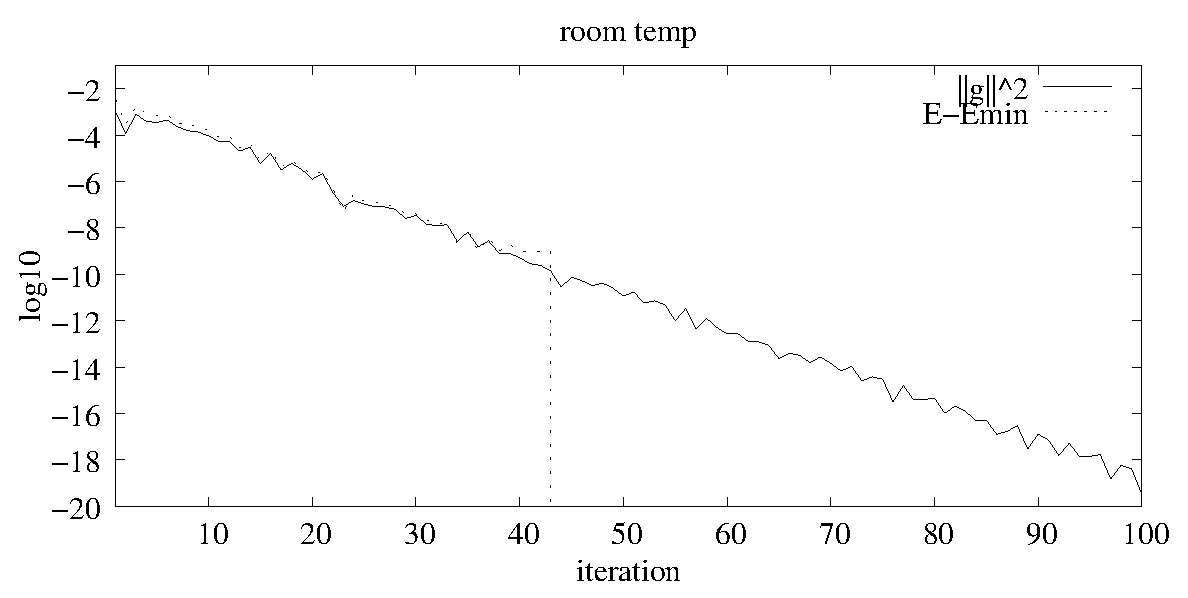
\includegraphics[height=3in]{cvg_room.eps}
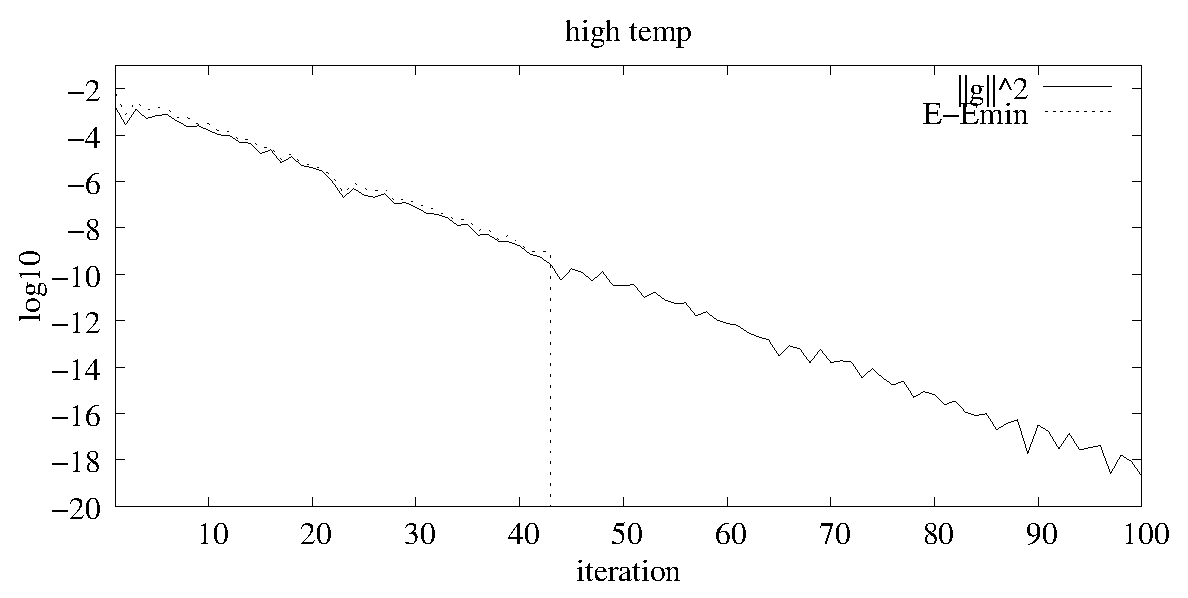
\includegraphics[height=3in]{cvg_1eV.eps}
\caption{The error in the energy, as well as the square-norm of gradient,
during the iterative minimization on a log scale.}
\label{energy_convergence}
\end{figure}

The OEP is found by using the gradient to iteratively minimize the energy.  We implemented this
minimization using Chebyshev acceleration on the fixed point equation
$x_{i+1} = x_i + \tau \nabla f(x_i)$ for some fixed $\tau$ empirically chosen.
The convergence of the energy of our test
system during this process is shown in Fig.~\ref{energy_convergence}.  The errors
in the energy were evaluated by comparing the energies obtained during the iterative minimization
to the result of a highly converged self-consistent calculation.  The convergence demonstrates
that the iterative OEP and self-consistent approaches give the same result, as would be expected
for the LDA energy functional.  The convergence is only weakly dependent on the electronic
temperature.  The asymptotic rate of convergence obtained in the iterative OEP approach is
not as rapid as the highly optimized mixing methods typically used in self-consistent calculations,
but a reasonable accuracy for practical purposes ($10^{-4}$ Ry.) can be obtained easily.

\section{Discussion}

We have found and verified an expression for the gradient of the Kohn-Sham energy with
respect to the local potential appearing in the Kohn-Sham Hamiltonian.  Our derivation
based on the density matrix naturally provides a result that is valid at finite temperature.
The cost of evaluating the optimized effective potential using this approach should be
comparable to the cost of a traditional density functional calculation using standard
functionals such as the LDA or GGA, but a greatly extended family of exchange-correlation
functionals that have an explicit dependence on the Kohn-Sham orbitals can be considered.

%\bibliographystyle{abbrv}
%\bibliography{/home/r1/lippert/REF/ref}

\begin{thebibliography}{1}

\bibitem{KohnSham:65}
W.~L. Kohn and L.~J. Sham, Phys. Rev. {\bf 140}, A1133 (1965).

\bibitem{HohenbergKohn:64}
P. Hohenberg and W. Kohn, Phys. Rev. {\bf 136}, B864 (1964).

\bibitem{TalmanShadwick:76}
J.~D. Talman and W.~F. Shadwick, Phys. Rev. A {\bf 14}, 36 (1976).

\bibitem{SahniGruenebaumPerdew:82}
V. Sahni, J. Gruenebaum, and J. P. Perdew, Phys. Rev. B {\bf 26}, 4371 (1982).

\bibitem{EngelVosko:93}  E. Engel and S.~H. Vosko, Phys. Rev. A {\bf 47}, 2800 (1993);
Phys. Rev. B {\bf 50}, 10498 (1994).

\bibitem{GorlingLevy:94}
A. G\"{o}rling and M. Levy, Phys. Rev. A {\bf 50}, 196 (1994).

\bibitem{Kotani:95}
T. Kotani, Phys. Rev. Lett. {\bf 74}, 2989 (1995).

\bibitem{StadeleMajewskiVoglGorling:97}
M. St\"{a}dele, J.~A. Majewski, P. Vogl, and A. G\"{o}rling, Phys. Rev. Lett. {\bf 79}, 2089 (1997);
M. St\"{a}dele, M. Moukara, J.~A. Majewski, P. Vogl, and A. G\"{o}rling, Phys. Rev. B {\bf 59},
10031 (1999).

\bibitem{Gorling99}
A. G\"{o}rling, Phys. Rev. Lett. {\bf 83}, 5459 (1999).

\bibitem{HymanStilesZangwill:00}
R.~Hyman, M.~Stiles, , and A.~Zangwill.
\newblock A gradient search method for orbital-dependent charge-density and
  current density functional calculations.
\newblock {\em Phys. Rev. B}, 62(23):15521--15526, 2000.

\bibitem{KummelPerdew:03}
S.~K\"{u}mmel and J.~P. Perdew.
\newblock Simple iterative construction of the optimized effective potential
  for orbital functionals, including exact exchange.
\newblock {\em Phys. Rev. Letters}, 90(4):043004, 2003.

\bibitem{HornJohnson.book:91}
R.~A. Horn and C.~R. Johnson.
\newblock {\em Topics in Matrix analysis}.
\newblock Cambridge University Press, Cambridge, 1991.

\bibitem{minres}
C.~C. Paige and M.~A. Saunders.
\newblock Solution of sparse indefinite systems of linear equations.
\newblock {\em {SIAM} J. Numer. Anal.}, 12:617--629, 1975.

\bibitem{GolubVanLoan.book:89}
G.~H. Golub and C.~F.~V. Loan.
\newblock {\em Matrix Computations}.
\newblock Johns Hopkins University Press, Baltimore, Maryland, 2d edition,
  1989.

\end{thebibliography}

\end{document}

